\subsection{Subspace identification for LDS models can be used as a foundation for a fast SLDS estimation procedure}
\label{sec:slds:3.2.5}
While the SLDS offers clear performance benefits over the AR-HMM, one significant drawback is the greater time and compute requirements needed to fit sLDS models. This is primarily due to the increase in the dimensionality of the parameter space, given the additional layer of (often high-dimensional) continuous latents as well as the need to jointly infer the discrete and continuous state sequences. Here, we provide a framework for an approach that can greatly speed up sLDS fitting time. This framework is founded on a mathematical concept called subspace identification (SSID), which aims to identify the system parameters of linear time invariant models by manipulating the structure of the output data (or input-output data, in the case of driven models) into a form that allows for the derivation of the model parameters \cite{ho_editorial_1966, van_overschee_n4sid_1994, viberg_subspace-based_1995, van_overschee_subspace_1996}. The general protocol involves organizing the data into Hankel matrices \cite{widom_hankel_1966} and then using one of a few variants of SSID to either (1) estimate the latent state sequence and subsequently recover the parameters using regression techniques or (2) decompose the Hankel matrix into constituent parts from which the system parameters can be extracted directly. We discuss the theory behind SSID and the steps in this process more thoroughly for both Gaussian-distributed data (which is relevant here) and other distribution classes in Chapter \ref{ch:bestlds}. 

The idea behind our method, called Fast Approximation using Subspace Techniques for Switching Linear Dynamical Systems (fastSLDS), involves taking subsets of output data (i.e. the observations in an SLDS model) that could reasonably be associated with different discrete states (i.e. behaviors), separately identifying the linear-Gaussian LDS system parameters associated with each data subset using SSID, and then taking the combined set of the recovered LDS parameters as estimates of the SLDS model parameters. The estimates can then be used as initializations for fitting the model using EM in order to infer the true parameters with greater accuracy (Fig. \ref{fig:slds:5}a).    
\begin{figure}[h!]
  \begin{center}
    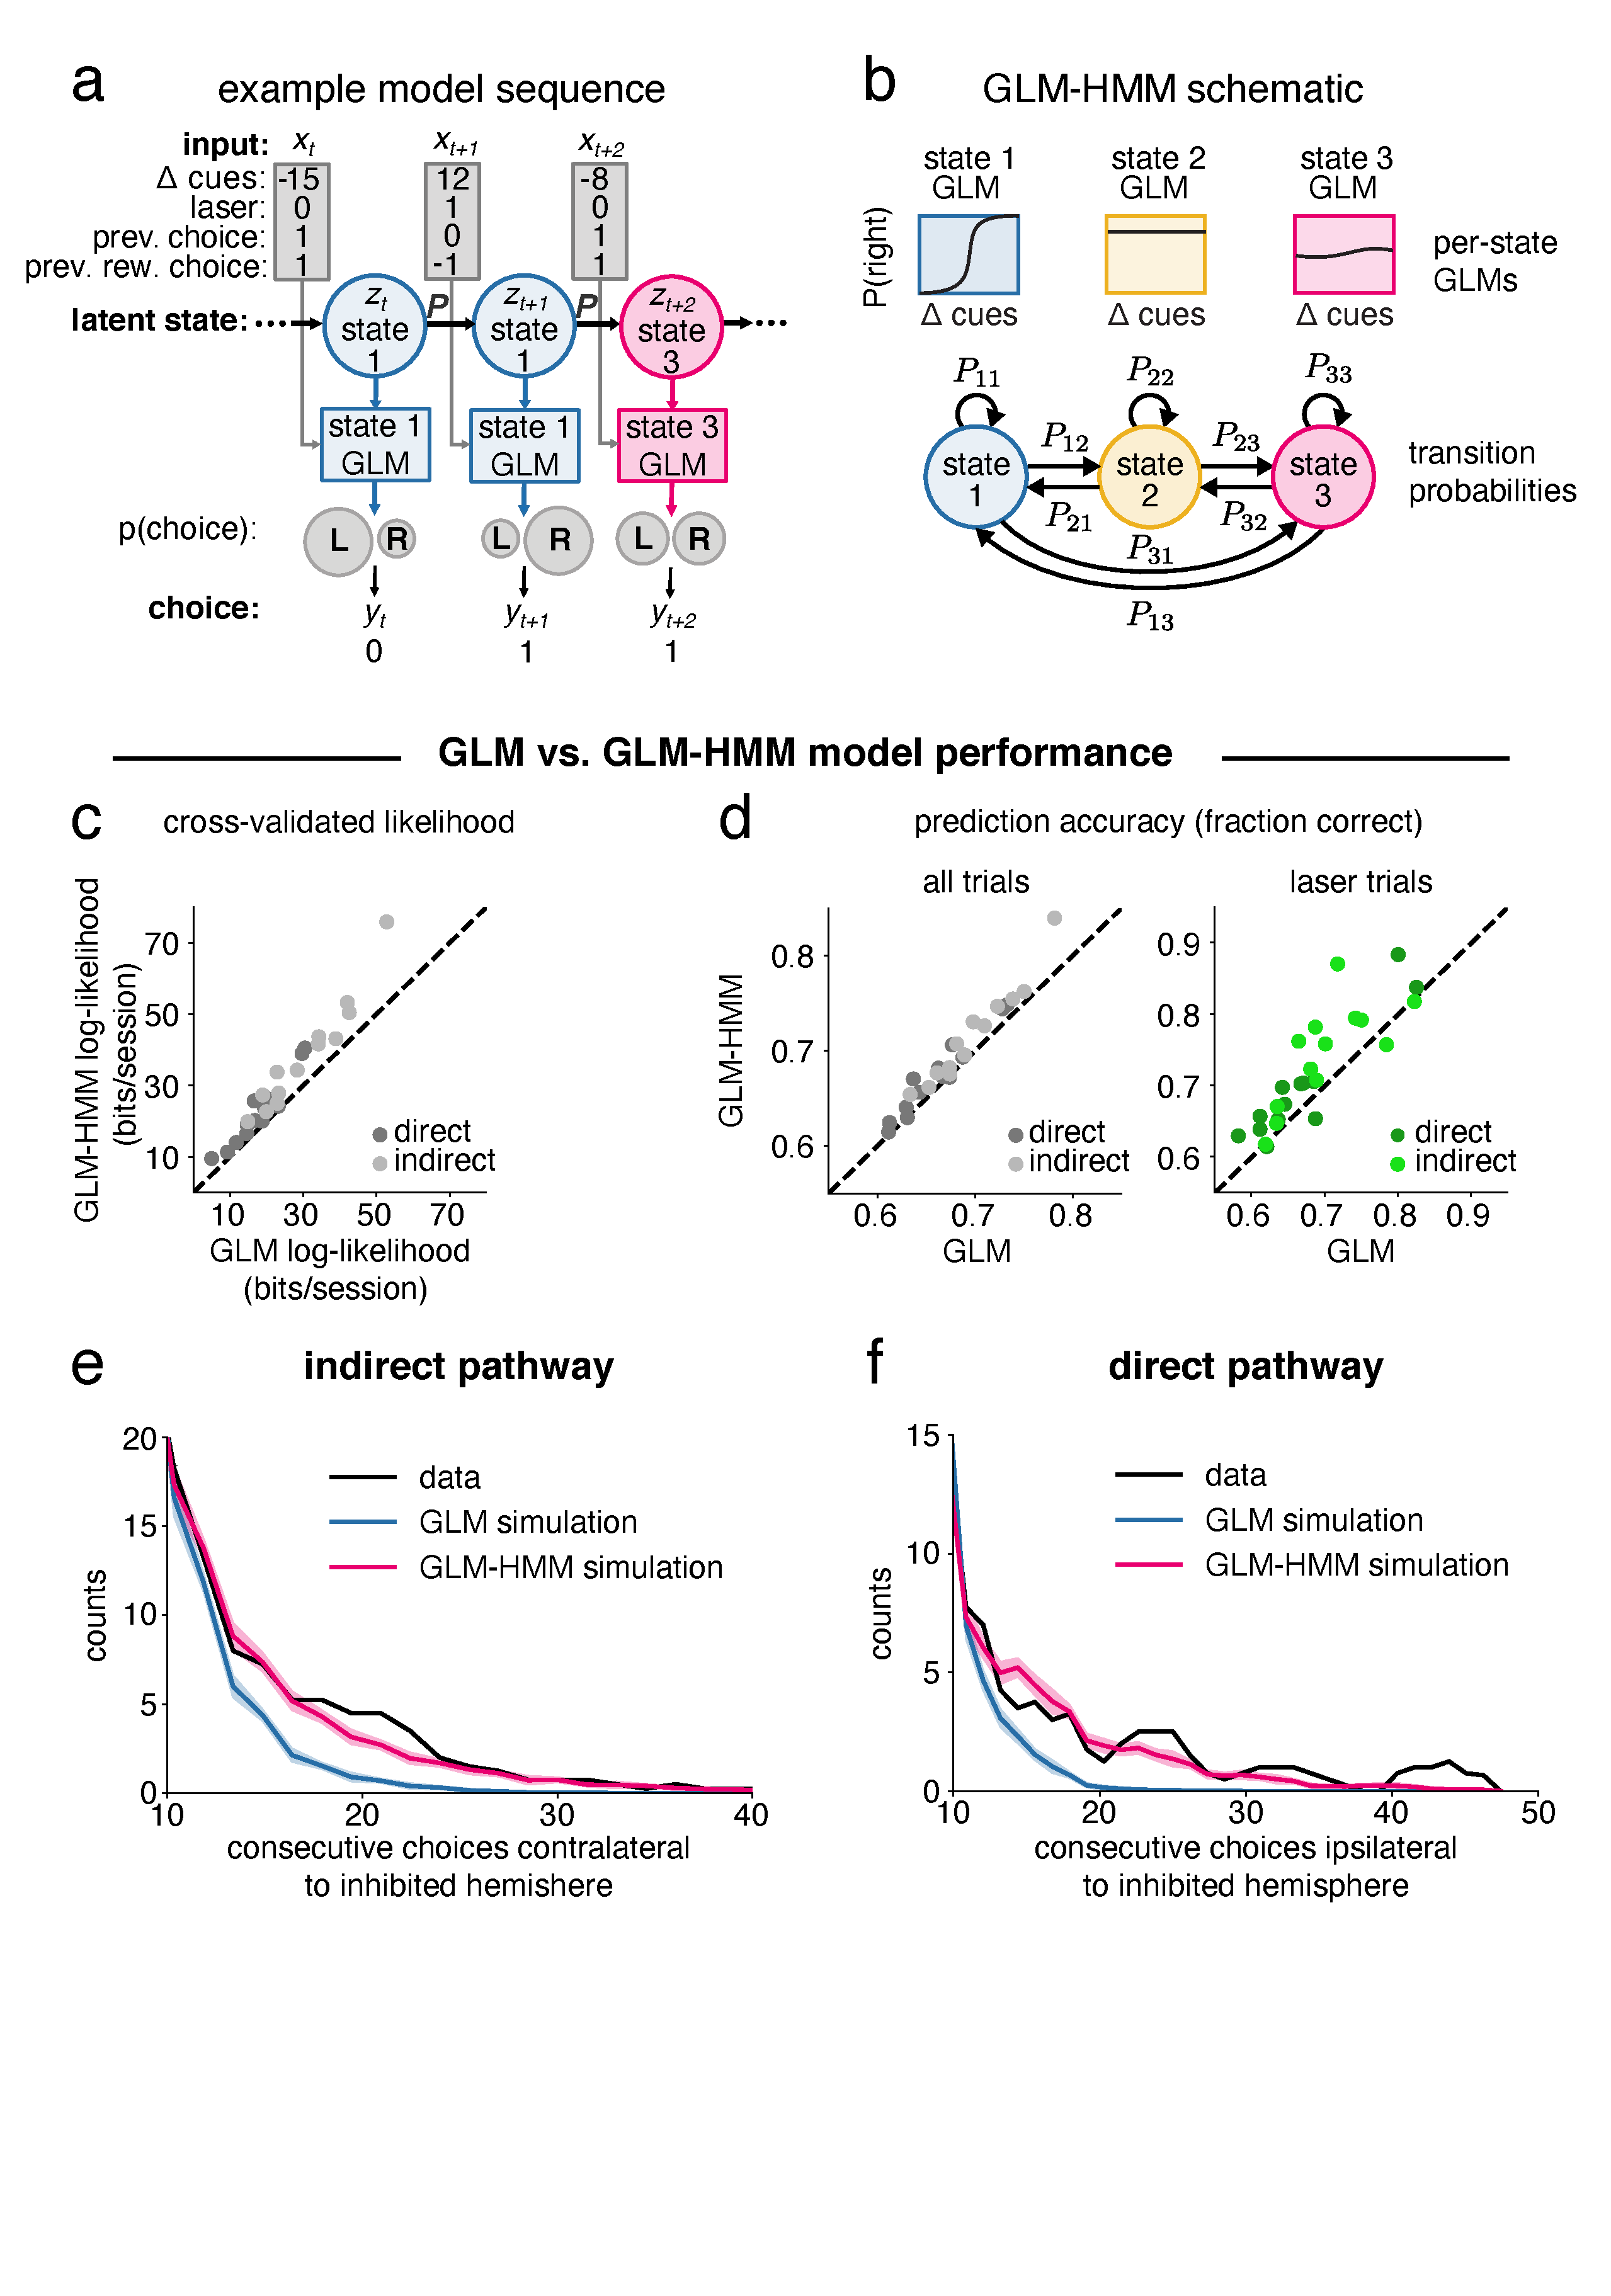
\includegraphics[width=0.90\linewidth]{ch3-slds/slds-figures/Fig5.pdf}
    \caption[A proposed procedure for using subspace identification to estimate the SLDS system parameters in a natural behavior context]{\textbf{A proposed procedure for using subspace identification to estimate the SLDS system parameters in a natural behavior context.}(a) fastSLDS schematic. Animal behavior is labeled at each frame of the video as either sitting, walking, or rearing (first row). We then combined all the labeled data associated with each behavior to create three datasets, each of which is a subset of the entire dataset (second row). Next, we fit an LDS to each behavior-specific dataset (third row), with the idea that the recovered parameters can then be combined to estimate the parameters for a 3-state SLDS (fourth row). (b) Visualization of the procedure for automatically labeling the data for one video. We used joint position coordinates (gray lines) to identify subsets}
    \label{fig:slds:5}
  \end{center}
  \vspace{-1.0cm}
\end{figure}

\begin{figure}[t!]
  \contcaption{of the data (black lines) corresponding to the desired behaviors using thresholding techniques (rearing: neck z position below 170, walking: velocity above 2, sitting: everything else) and automatically labeled the behaviors accordingly (``auto labels", second row, labels are in the darker color). To validate our choice of thresholds, we compared the automatic labels to hand labels (last row) for one video and after optimizing performance (automatic to hand label match rate for sitting: 84\%, walking: 89\%, rearing: 94\%), applied the thresholding to generate automatic labels across all videos.}% Continued caption
\end{figure}



To quickly identify subsets of data that could reasonably be associated with different states in the natural behavior context, we created a course automatic detection technique by thresholding the uncentered, unrotated keypoint data under different conditions for different behaviors (Fig. \ref{fig:slds:5}b). For example, we identified frames in which the mouse was rearing as frames in which the animal's head position (taken as the z position of the neck keypoint) exceeded a specified threshold. We determined the appropriate thresholds by comparing the automatic labels to those of hand labels for one video (in which frames were manually assigned to each behavior through visual inspection) and adjusted the threshold values until the fraction of automatic labels that matched the hand labels was maximized. 